\section{Introduction to Tools}
% -----------------------------------------------------------------------
\subsection{Basic Tools}
\begin{frame}{Tools?}
\begin{itemize}
\item \emphbf{Practical implementation} implies a number of \emphbf{choices} in terms of framework or software to use.
For example:
\item Programming language: Python
\item Deep learning library: PyTorch
\item and more...
\item This section: introduction to these practical \textit{tools}.
\end{itemize}
% PyCharm: demo. Very convenient for both reading and writing!
\end{frame}

\begin{frame}{Python}
\begin{itemize}
\item Again: if you are not familiar with Python, check: \link{https://docs.python.org/3/tutorial/}
\item High-level, general purpose, programming language
\begin{itemize}
\item[-] ``easy to use", "broadly popular"
\item[-] The most popular language for deep learning today
\item[-] Many libraries are available.
\item[-] A few characteristics:\\ \textit{indentation} is part of syntax, dynamically typed, indices start from 0... etc
\end{itemize}
\item \alertbf{Version} to be used: Python 3.6+.
\item You will still find Python 2.x code... \\
But for any new code use: Python 3.6+.
\end{itemize}
% PyCharm: demo. Very convenient for both reading and writing!
\end{frame}

\begin{frame}[fragile]{Python, simple illustration}
\vspace{-5mm}
%Bubble sort\footnote{taken from {\scriptsize \url{https://realpython.com/sorting-algorithms-python/}}}:
\begin{python}
def bubble_sort(list_nums):
    # Implement Bubble Sort.
    already_sorted = True
    numbers = list_nums.copy()
    n = len(numbers)
    for i in range(n):
        for j in range(n-i-1):
            if numbers[j] > numbers[j+1]:
                numbers[j], numbers[j+1] = numbers[j+1], numbers[j]
                already_sorted = False
        if already_sorted:
            break
    return numbers
\end{python}
\pause
\begin{python}
>>> my_numbers = [58, 37, 2, 11, 96, 15, 64]
>>> bubble_sort(my_numbers)
[2, 11, 15, 37, 58, 64, 96]
\end{python}
\pause
Though you should use \textbf{built-in} function instead (more efficient).
\begin{python}
>>> sorted(my_numbers)
[2, 11, 15, 37, 58, 64, 96]
\end{python}
\end{frame}

\begin{frame}[fragile]{Python, simple illustration 2}
\vspace{-5mm}
\textbf{Loops} in Python are very simple (check Sec.~5.6 in the tutorial)
\begin{python}
# dictionary storing count of fruits.
>>> basket = {'apple': 4, 'banana': 2, 'orange': 5}
>>> for fruit, count in basket.items():
...   print(fruit, count)
... 
apple 4
banana 2
orange 5
\end{python}
\pause
\begin{python}
# loop over a list, with loop counter:
>>> for i, v in enumerate(['tic', 'tac', 'toe']):
...     print(i, v)
...
0 tic
1 tac
2 toe
\end{python}
\end{frame}

\begin{frame}[fragile]{Python, many packages}
\vspace{-3mm}
\textbf{Different packages} provide you with useful functions.\\
\vsp
E.g. \code{math} module for quick calculations:
(e.g. you want to immediately know the log of some number!)
\begin{python}
>>> import math
>>> math.log(0.1)
-2.3025850929940455
>>> y = math.log(0.1)
>>> z = math.exp(y)
>>> z
0.10000000000000002
\end{python}
\begin{itemize}
\item \textbf{NumPy} \code{numpy}: manipulation of multi-dimensional arrays.\\
\begin{itemize}
\item Seen in \emphbf{Exercise 1} !
\end{itemize}
\item \textbf{Matplotlib} \code{matplotlib}: tool for visualization, generate plots.
\begin{itemize}
\item More in \emphbf{Exercise 2} !
\end{itemize}
\item etc...
\end{itemize}
\end{frame}

\begin{frame}[fragile]{Python, package installer}
\vspace{-3mm}
The basic \textbf{package installer} for Python is \code{pip} (or \code{pip3} or Python 3).\\
\vsp
\begin{itemize}
\item To install the latest version of ``SomeProject”:\\
\begin{python}
pip3 install "SomeProject"
\end{python}
\item To install a specific version (e.g. version 1.1):\\
\begin{python}
pip3 install "SomeProject==1.1"
\end{python}
\end{itemize}
%Alternatively: If you can use \textbf{Anaconda/Miniconda}, see e.g.:
%\link{https://docs.conda.io/projects/conda/en/latest/user-guide/concepts/installing-with-conda.html}\\
%(\code{conda} is very convenient for environment managing; see later slides).
\end{frame}

\begin{frame}{Code Style}
\vspace{-3mm}
\textbf{Need guidelines to write consistent (easy to read) code.}
\begin{itemize}
\item How should I name my function? my variable? class?
\item How should I space? indent? comment?
\item What is the longest acceptable line length?\\
\item How to split long lines... etc!
\end{itemize}
\vsp
\textbf{Some reference guidelines:}\\
\begin{itemize}
\item PEP 8
\link{https://www.python.org/dev/peps/pep-0008/}
\item Google guideline
\link{https://github.com/google/styleguide/blob/gh-pages/pyguide.md}
\end{itemize}
\vsp
\textbf{Crucial importance for collaborative projects!}\\
\begin{itemize}
\item When you ask other people to \textbf{review} your code.
\item But also for yourself (to ease reading your own code).\\
\item \emphbf{Consistent} formatting makes reading much easier.
\end{itemize}
\end{frame}

\begin{frame}{Editor (for Python)}
\textbf{Up to you!}
\begin{itemize}
\item Emacs, vim, nano, kate, VSCode, ...\\
\item If you do not know, you can try \textbf{VSCode} or \textbf{PyCharm} (Community).
\begin{itemize}
\item Very convenient for both reading (navigating through a large project) and writing (with less formatting errors).
\end{itemize}
\item What I use: vim (for simple edits) and VSCode in general.
\end{itemize}
\end{frame}

\begin{frame}{Managing environment}
\textbf{(Excursion; no need to worry about this in this course)}
\vsp
\begin{itemize}
\item Python, libraries, softwares, ... evolve over time.
\item Resulting in code with \emphbf{different versions} for each tool.
\begin{itemize}
\item[-] Currently working code has no guarantee to work again in another environment.\\
\item[-] Also: often you will be using code that you find on the internet (Github), that someone had written, you do not know when, which requires some specific sets of versions for libraries...
\end{itemize}
%\item You might need to create a specific set of these packages
%in order to be able to run many different code/software.
%demo.
\end{itemize}
\vsp
\emphbf{Environment managing tools} can help handling multiple configurations.
\begin{itemize}
\item Typical tools: \code{virtualenv}, \code{conda}
\item If you do not have any preference yet, try Miniconda.\\
\begin{itemize}
\item[-] \link{https://docs.conda.io/en/latest/miniconda.html}
\item[-] \link{https://docs.conda.io/projects/conda/en/latest/user-guide/tasks/manage-environments.html}
\end{itemize}
\end{itemize}
% Example: \codeb{conda activate DL-lab} in your ICS script.
\end{frame}

%\begin{frame}{Managing environment (cont'd)}
%\begin{itemize}
%\item Basically: you want to maintain multiple sets of packages with their correct versions.\\
%\item Typical tools: \code{virtualenv}, \code{conda}
%\item If you do not have any preference yet, try Miniconda.
%\begin{itemize}
%\item \link{https://docs.conda.io/en/latest/miniconda.html}
%\item \link{https://docs.conda.io/projects/conda/en/latest/user-guide/tasks/manage-environments.html}
%\end{itemize}
%\end{itemize}
%\emphbf{demo?}
%\end{frame}

\begin{frame}{Other useful tools}
\begin{itemize}
\item Internet and Google!
\item Very likely, the same problem you encountered has been already solved by other people!
\item Search your problem, and you might find solutions on e.g. \textit{StackOverflow}.
\item Be careful with version mismatch.
\end{itemize}
\end{frame}

\begin{frame}{Libraries for Deep Learning}
\vspace{-3mm}
\textbf{Many possibilities, different teams/companies.}
\begin{itemize}
\item TensorFlow (Google), MXnet (Amazon), JAX (Google),...
\item Other high-level framework: keras (Google), ...
\end{itemize}
\pause
\vsp
\textbf{Side notes:}
\begin{itemize}
\item Theano (UdeM): end of support in 2017.
\item Chainer (Preferred Networks): migration to PyTorch in 2019.
\item Caffee (Berkeley, Facebook) merged to PyTorch in 2018. 
\item Cognitive Toolkit (Microsoft): 2016-2017.
\item even older... Quicknet (Berkeley)
\end{itemize}
\pause
\vsp
This lecture: \textbf{PyTorch}
\begin{itemize}
\item Development led by Meta/Facebook AI Research.
\item Last week: became a project under Linux Foundation
\item Very popular already. Increasing popularity...
\item Used for example by OpenAI, Tesla...
\end{itemize}
\end{frame}
% \subsection{Introduction to PyTorch}

\begin{frame}[fragile]{Introduction to PyTorch}

\textbf{Two core aspects:}
\vsp
\begin{itemize}
\item GPU-friendly tensors.
\item Automatic differentiation.
\end{itemize}
\vsp
Note: current version PyTorch 1.12.1 (Aug. 2022) \sout{PyTorch 1.9.0 (June 2021)} \sout{PyTorch 1.6.0 (July 2020)} \\
%\begin{python}
%import torch
%\end{python}
\end{frame}

\begin{frame}{Introduction to PyTorch (cont'd)}
\textbf{Packages which you will be often importing:}\\
\begin{itemize}
\item \codeb{torch}: top-level package.
\item \codeb{torch.nn}: modules for building neural networks. 
\item \codeb{torch.nn.functional}: various functions.
\item \codeb{torch.optim}: optimization related tools. 
\item \codeb{torch.utils}: handling data etc.
\item ...
\end{itemize}
Many examples later.
\end{frame}

% \subsection{Introduction to PyTorch}
\begin{frame}{Introduction to PyTorch (cont'd)}
\textbf{Many packages are available.}\\
\vsp
E.g.~to work with:
\begin{itemize}
\item image: \codeb{torchvision}
\item audio: \codeb{torchaudio}
\item text: \codeb{torchtext}
\item ...
\end{itemize}
\vsp
\end{frame}

\begin{frame}{Tensors}
\pause
\textbf{These are all tensors.}
\vspace{5mm}
  \begin{center}
    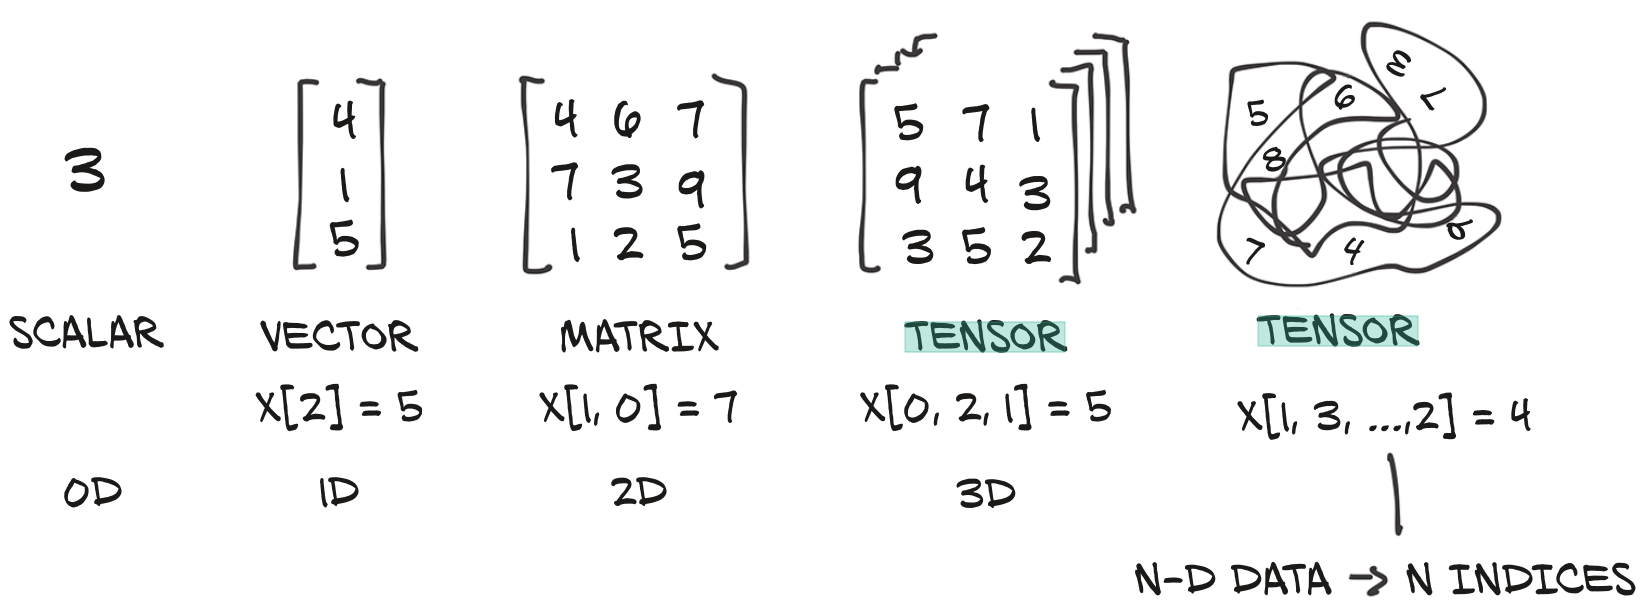
\includegraphics[height=0.5\textheight]{figures/tensors.png}
  \end{center}
\textbf{Including those with a rank of 0, 1 and 2, which have common names:\\ scalar, vector, matrix.}\\
\vspace{5mm}
\scriptsize{Figure taken from \citem{pytorchbook2020}.}\\
\end{frame}

\begin{frame}{Tensors (cont'd)}
\textbf{You will be manipulating multi-dimensional arrays all the time:}
\vsp
\begin{itemize}
\item You have an image.\\ It has height, width, and color channels (each pixel represented by red-green-blue): it's a 3d-array.\\ You have multiple images: you get a 4d-array.
\pause
\item You have a written sentence. \\You replace each word in the sentence by its ID, you get a 1d-array.\\ You have multiple sentences; you get a 2d-array.\\ (some subtlety w/ handling various sentence lengths)
\pause
\item These are all \emphbf{tensors}.
\end{itemize}
\vsp
Corresponding class in PyTorch is \codeb{torch.Tensor}.\\
Similar to NumPy's \codeb{numpy.ndarrays}.
\end{frame}

\begin{frame}[fragile]{Tensors, basic concepts}
\vspace{-7mm}
\codeb{torch.tensor} function creates \codeb{torch.Tensor} object:
\begin{python}
>>> import torch
>>> x = torch.tensor([[1, 2], [3, 4]])
>>> x
tensor([[1, 2],
        [3, 4]])
\end{python}
\pause
A fundamental attribute is the \emphbf{shape} of tensor:
\begin{python}
>>> x.shape  # or `x.size()`
torch.Size([2, 2])
\end{python}
\pause
Also: every \codeb{torch.Tensor} has \codeb{dtype} (data type) attribute.
\vspace{-1mm}
\begin{python}
>>> x.dtype
torch.int64
>>> x = torch.tensor([[1, 2], [3, 4]], dtype=torch.float32)
>>> x
tensor([[1., 2.],
        [3., 4.]])
>>> x.dtype
torch.float32
\end{python}
\end{frame}

\begin{frame}[fragile]{Tensors (cont'd)}
\vspace{-7mm}

You can create some classic/random tensors using e.g.
\begin{itemize}
\item  \codeb{eye} (diagonal tensor), \codeb{zeros} (all-zero tensor), \codeb{ones} (all-one tensor), \codeb{arange} (1D tensor with incrementally increasing integers),
\codeb{rand} (random tensor),... by specifying the shape/size you want.
\end{itemize}
\begin{python}
>>> x = torch.ones([2, 3])
>>> x
tensor([[1., 1., 1.],
        [1., 1., 1.]])
\end{python}
\begin{python}
>>> x = torch.rand([2, 3])
>>> x
tensor([[0.9332, 0.0222, 0.0364],
        [0.7155, 0.8362, 0.9795]])
\end{python}
\end{frame}

\begin{frame}[fragile]{Tensors, \\conversion from/to NumPy ndarrays.}
Simply: \codeb{torch.from\_numpy()} and \codeb{x.numpy()}
\begin{python}
>>> import numpy
>>> import torch
>>> a = numpy.array([1, 2, 3])
>>> a
array([1, 2, 3])
>>> b = torch.from_numpy(a)
>>> b
tensor([1, 2, 3])
>>> b.numpy()
array([1, 2, 3])
\end{python}

\end{frame}

\begin{frame}{Tensors,\\ manipulating dimensionality}
\textbf{Checking the shape of tensor:}
\begin{itemize}
\item \codeb{x.size()}  return tuple-like object of shape.
\item \codeb{x.shape}  same as above (alias).
\item \codeb{x.ndim}  return number of dimensions
\end{itemize}
\vsp
\pause
\textbf{Modifying the shape of tensor:}
\begin{itemize}
\item \codeb{x.view(a,b,...)}  return tensor; \textbf{reshape} of x to size (a,b,...) without copying.
\item \codeb{x.reshape(a,b,...)}  return tensor; \textbf{reshape} of x to size (a,b,...). (when you can not use \codeb{view}; you will know as PyTorch will complain).
\item  \codeb{x.permute(*dims)}  permute dimensions.
\item  \codeb{x.squeeze(dim)} \& \codeb{x.unsqueeze(dim)}  return tensor with removed/added axis.
\end{itemize}
\vsp
\pause
\textbf{Combining multiple tensors:}
\begin{itemize}
\item  \codeb{torch.cat}, \codeb{torch.stack}, to concatenate/ stack multiple tensors... etc!
\end{itemize}
\pause
\vsp
\emphbf{You will try them all in Exercise 2.}
\end{frame}

\begin{frame}[fragile]{Tensors, indexing / slicing}
\vspace{-7mm}
You can access a sub-tensor via indices (similar to NumPy).
\begin{python}
>>> y = torch.arange(15)
>>> y
tensor([ 0,  1,  2,  3,  4,  5,  6,  7,  8,  9, 10, 11, 12, 13, 14])
>>> y.size()
torch.Size([15])
>>> t = y.view(3,5)
>>> t
tensor([[ 0,  1,  2,  3,  4],
        [ 5,  6,  7,  8,  9],
        [10, 11, 12, 13, 14]])
>>> t.size()
torch.Size([3, 5])
>>> t[1, 3]
tensor(8)
>>> t[2, 1:3]
tensor([11, 12])
>>> t[0:2, :]
tensor([[0, 1, 2, 3, 4],
        [5, 6, 7, 8, 9]])
\end{python}
\end{frame}

\begin{frame}[fragile]{Tensors, example operations}
\vspace{-5mm}
Different types of \emphbf{operations}: 
\begin{itemize}
\item ``standard" math operations between two tensors.
\item operations which do something on a single tensor; e.g. along some axis/dimension.
\end{itemize}
\begin{python}
>>> x = torch.randint(low=0, high=10, size=[2, 3])
>>> y = torch.randint(low=0, high=10, size=[2, 3])
>>> x
tensor([[5, 1, 8],
        [4, 5, 9]])
>>> y
tensor([[1, 6, 9],
        [7, 4, 9]])
>>> x + y
tensor([[ 6,  7, 17],
        [11,  9, 18]])
>>> x * y
tensor([[ 5,  6, 72],
        [28, 20, 81]])
\end{python}
\end{frame}

\begin{frame}[fragile]{Tensors, more example operations}
\vspace{-5mm}
Element-wise function:
\begin{python}
>>> import torch.nn.functional as F
>>> z = torch.randint(low=-10, high=10, size=[2, 3])
>>> z
tensor([[ 0, -7, -4],
        [-9,  7,  2]])
>>> F.relu(z)
tensor([[0, 0, 0],
        [0, 7, 2]])
\end{python}
\vsp
Operation along some axis/dimension (here sum):
\begin{python}
>>> torch.sum(z)
tensor(-11)
>>> torch.sum(z, axis=0)
tensor([-9,  0, -2])
>>> torch.sum(z, axis=1)
tensor([-11,   0])
\end{python}
\end{frame}

\begin{frame}[fragile]{Tensors, broadcasting}
\vspace{-7mm}
What happens when sizes do not match?
\pause
\begin{python}
>>> a = torch.ones(2,1)
>>> a
tensor([[1.],
        [1.]])
>>> b = torch.ones(1,2)
>>> b
tensor([[1., 1.]])
>>> a + b
tensor([[2., 2.],
        [2., 2.]])
\end{python}
It ``guesses" the operation you intend to do: \textbf{broadcasting}.\\ 
\pause
Make sure that it's what you really want! Maybe you wanted:
\begin{python}
>>> a + b.t()  # b.t() is transpose of b.
tensor([[2.],
        [2.]])
\end{python} \link{https://pytorch.org/docs/stable/notes/broadcasting.html} to read more about it...
\end{frame}

\begin{frame}[fragile]{Tensors on GPU?}
% \vspace{-3mm}
 General purpose \textbf{graphical processing unit}, GPGPU or simply GPU.\\
\begin{itemize}
\item Hardware.
\item Accelerate many operations of linear algebra (such as matrix multiplication).
\item[-] Core computations in neural networks.
\item[-] In the past: low level implementation in \code{CUDA} had to be done.
\item[-] Now: straightforward using deep learning library (such as PyTorch). Users only need to write code in Python.
\end{itemize}
\begin{minipage}{0.45\linewidth}
\begin{figure}
                        \centering
                        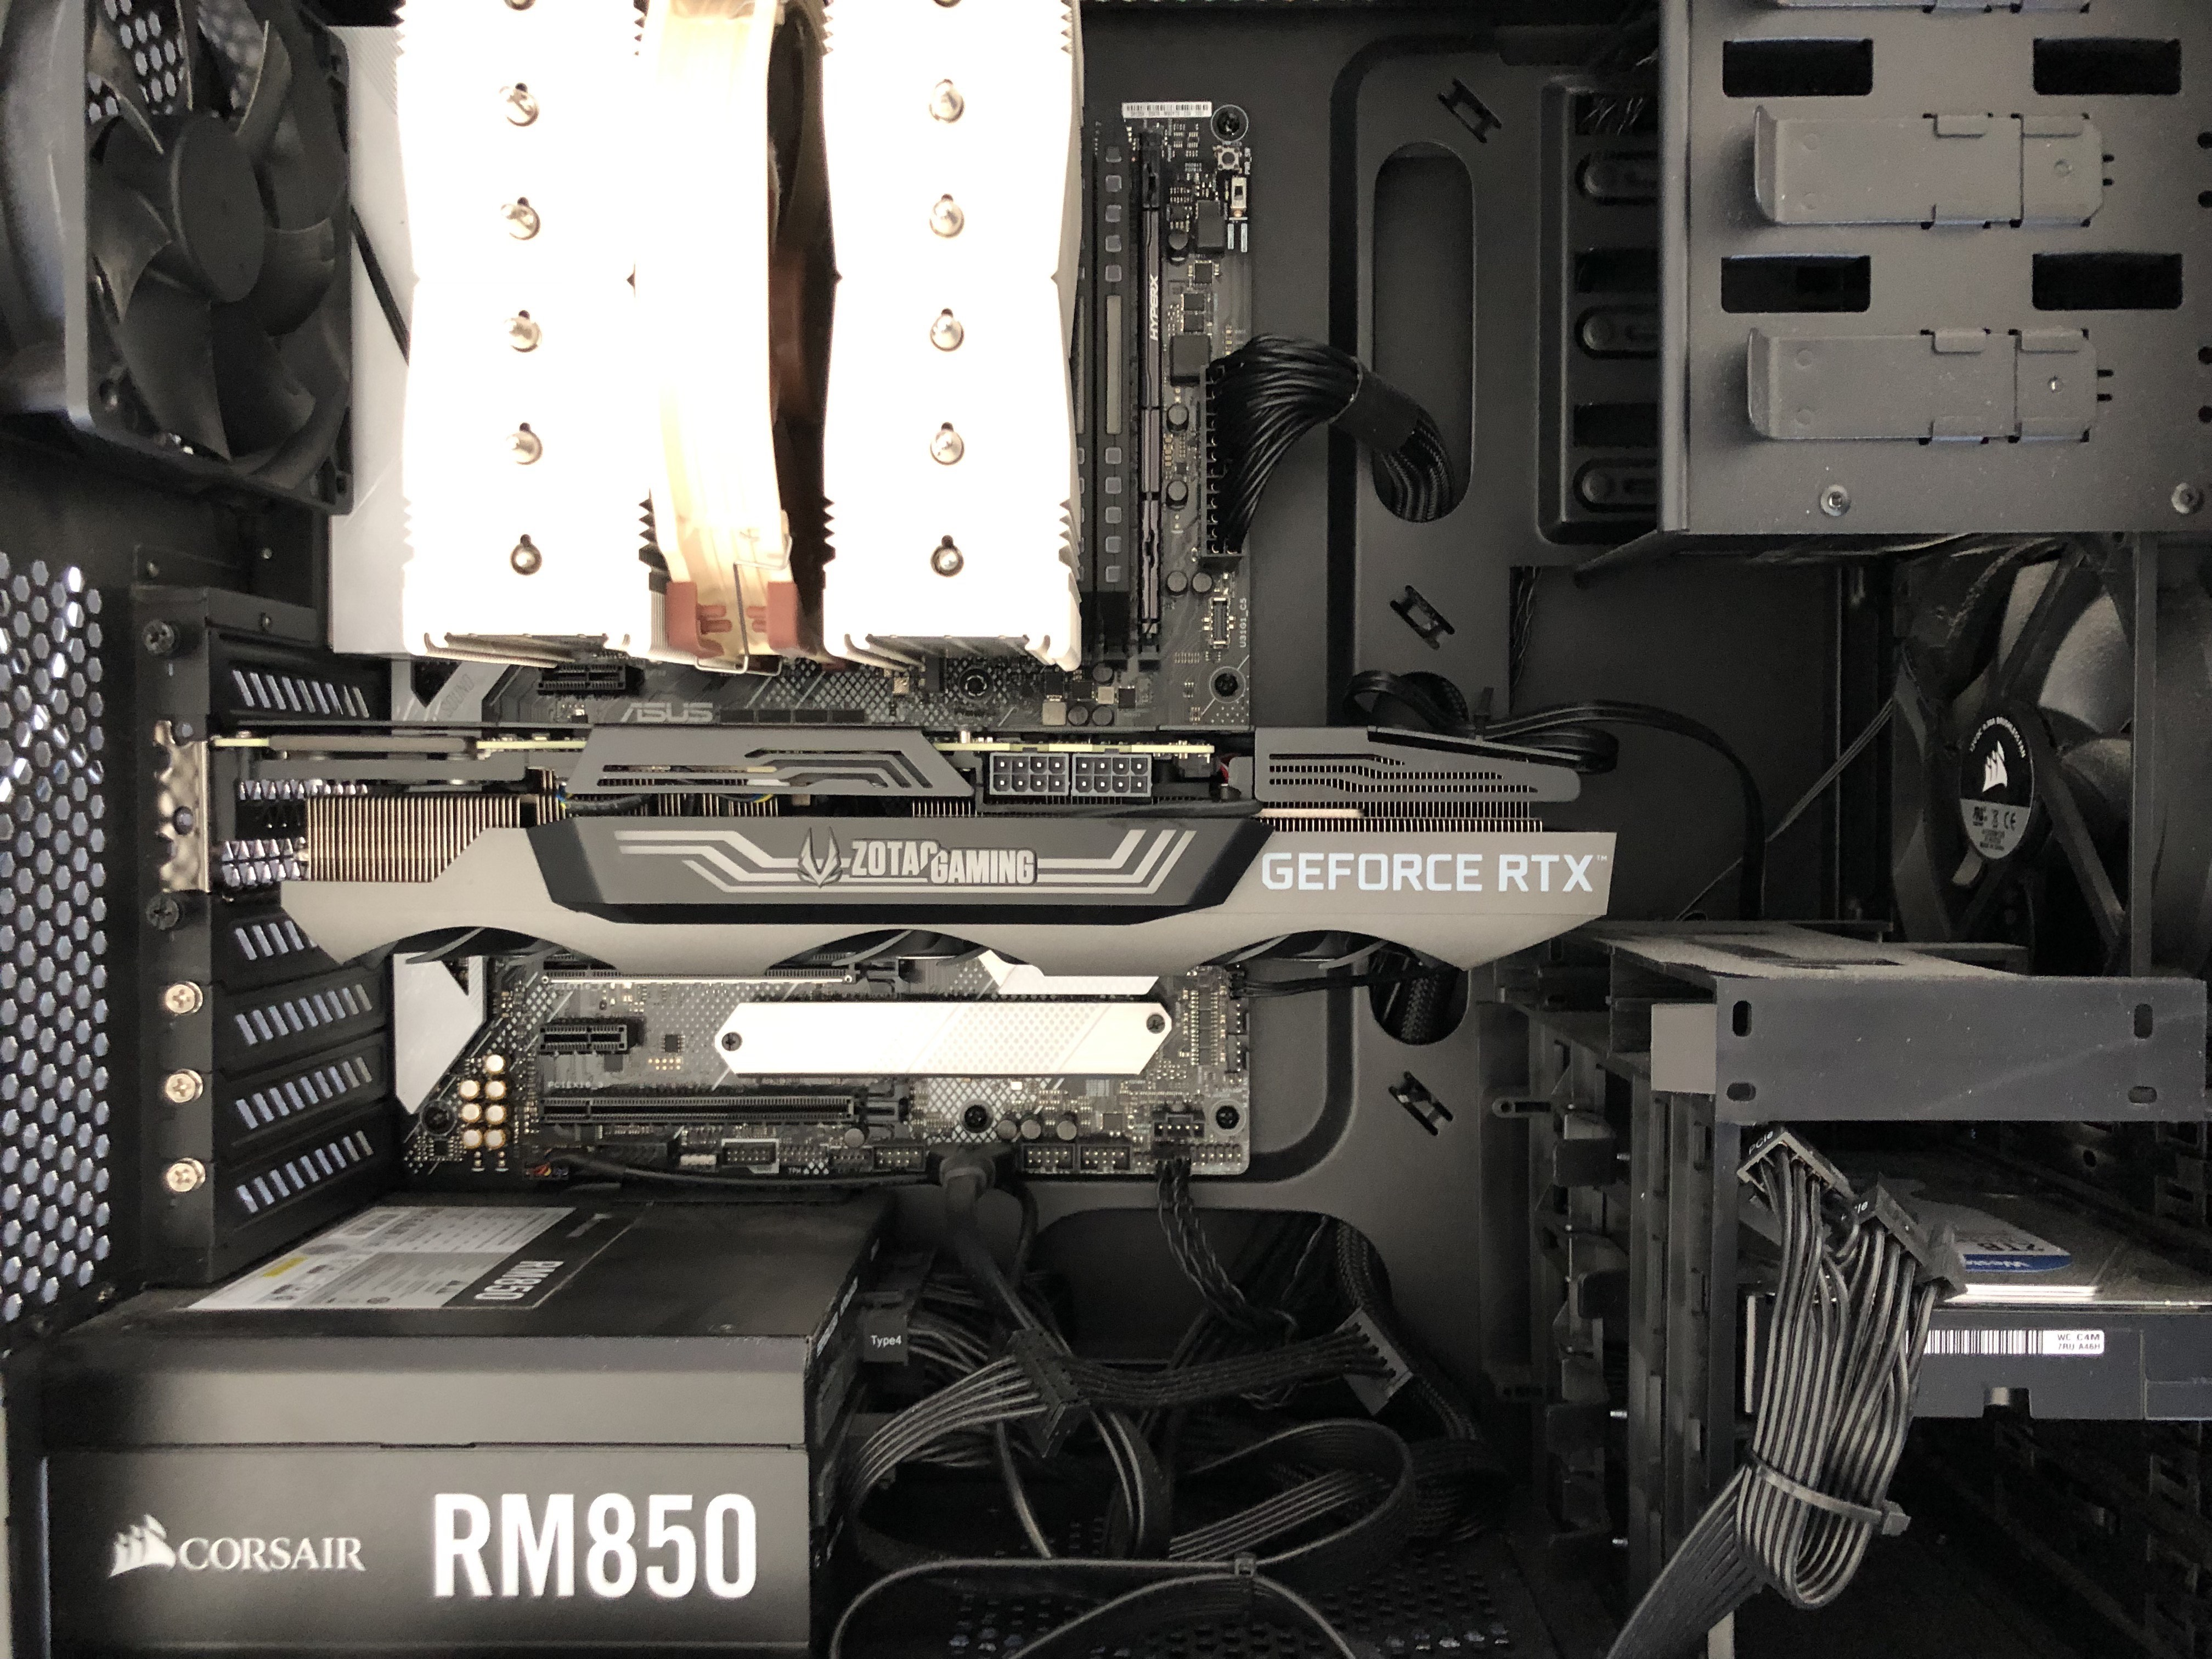
\includegraphics[width=.9\linewidth]{./figures/gpu_1.jpeg}
\end{figure}
\end{minipage}
\begin{minipage}{0.45\linewidth}
\begin{figure}
                        \centering
                        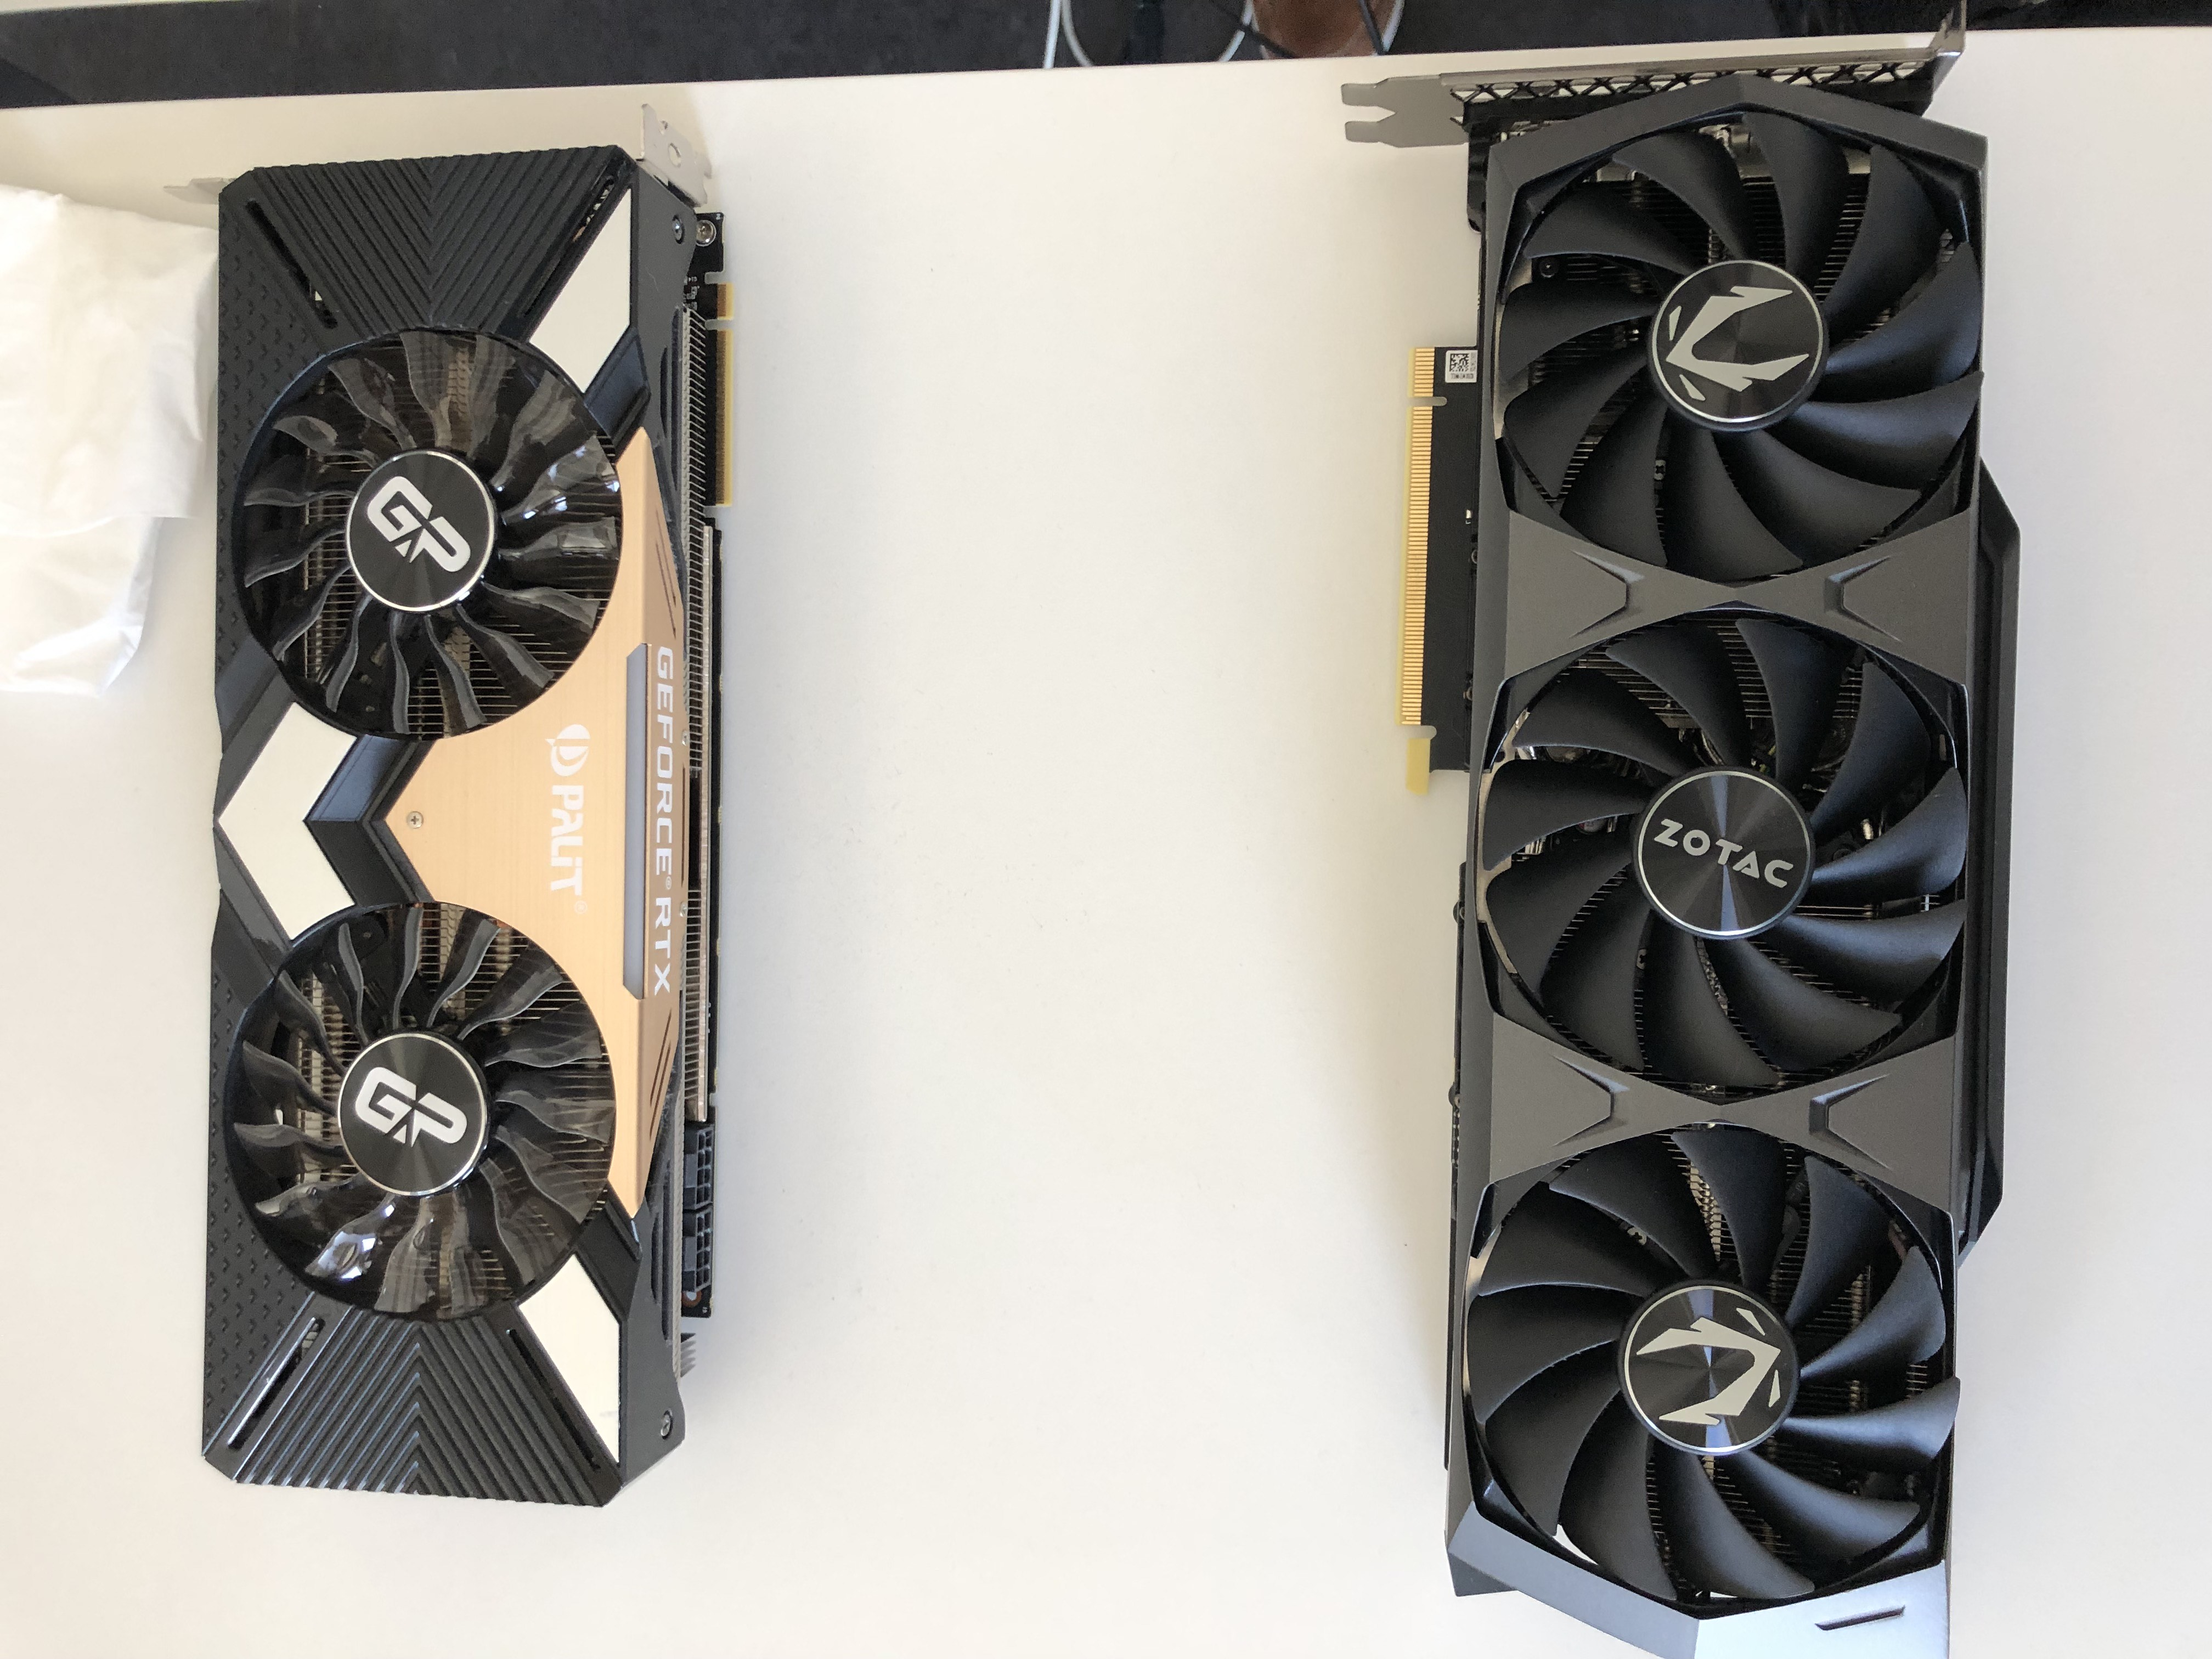
\includegraphics[width=.9\linewidth]{./figures/gpu_2.jpeg}
\end{figure}
\end{minipage}
\end{frame}

\begin{frame}[fragile]{Tensors on GPU? (cont'd)}
\vspace{-3mm}
Again: GPU is a hardware!\\
\begin{itemize}
\item To compute using GPU, you need to copy tensors to GPU memory.
\item Every \code{torch.Tensor} has the \code{device} attribute (basically CPU or GPU, tells the device on which the tensor is stored.).
\item Straightforward to transfer between devices in PyTorch \codeb{x.to(device)}:
\end{itemize}
\begin{python}
>>> device = torch.device(
...     "cuda:0" if torch.cuda.is_available() else "cpu")
>>> a = torch.rand([2, 3])
>>> a.device
device(type='cpu')
>>> b = a.to(device)  # copy to GPU.
>>> b.device
device(type='cuda', index=0)
\end{python}
\begin{itemize}
\item You can also directly create a tensor on a specific device \codeb{a = torch.rand([2, 3], device='cuda')}
\end{itemize}

NB: \codeb{to} is a method introduced after version $\geq$ 0.4.\\ (Used to be \code{x.cuda()} and \code{x.cpu()} before)
\end{frame}

\begin{frame}[fragile]{A few words on GPUs}
\vspace{-3mm}
\begin{itemize}
\item Different GPUs have different specs. Better GPUs released every year.
\item For example, on the USI's ICS cluster:
\begin{itemize}
\item NVIDIA GeForce GTX \textbf{1080} \textbf{8\,GB}
\item NVIDIA GeForce GTX \textbf{1080 Ti 11\,GB}
\item NVIDIA GeForce GTX \textbf{2080 Ti 11\,GB} (faster than 1080).
\end{itemize}
\item Be aware of the GPU memory of the machine.\\
Classic error you will get:\\
\codeb{RuntimeError: CUDA out of memory. Tried to allocate ...}
\item A typical solution is to reduce the batch size...
\item or run on machines which has more GPU memory.
\end{itemize}

\end{frame}

%\begin{frame}{Reminder: backpropagation}
%equations? illustrate it's painful to do it by hands?
%\end{frame}

\begin{frame}{Automatic differentiation}
Reminder: for gradient descent
$\theta(n+1) = \theta(n) - \alpha * \nabla_{\theta} \mathcal{L}(\theta(n))$\\
you need to compute the \textbf{gradient} of the loss $\nabla_{\theta} \mathcal{L}(\theta(n))$ w.r.t. the model parameters. Need to do backpropagation!\\
\vsp
\vsp
In PyTorch, this computation is \textbf{automatic}:
\begin{itemize}
\item Write computations of a scalar \codeb{loss} as a function of some tensors.
\item \codeb{loss.backward()} computes \textit{all} gradients\\ i.e. \textbf{no need to write these computations by yourself}.
\item \textit{all}? Every \codeb{torch.Tensor} has \codeb{requires\_grad} attribute.
\end{itemize}
\vsp
If interested in learning how this works; see e.g. \link{https://www.youtube.com/watch?v=MswxJw-8PvE}
\end{frame}

\begin{frame}[fragile]{Automatic differentiation (cont'd)}
Illustration:
\begin{python}
>>> import torch
>>> x = torch.tensor(2, requires_grad=True, dtype=torch.float32)
>>> x
tensor(2., requires_grad=True)
>>> y = torch.tensor(3, requires_grad=True, dtype=torch.float32)
>>> z = x * x + y  # Forward computation.
>>> z.backward()  # "dz/dx = 2 x"
>>> x.grad
tensor(4.)
\end{python}
\end{frame}

\begin{frame}[fragile]{Automatic differentiation (cont'd)}
\vspace{-3mm}
Note: gradients are accumulated.\\
Continue from the previous slide:
\begin{python}
>>> a = x * x + y  # define one more tensor.
>>> a.backward()  # add "da/dx" to "x.grad"
>>> x.grad  # contains "dz/dx + da/dx"
tensor(8.)
\end{python}
If this is not wanted, you need to reset it:
\begin{python}
>>> x.grad.data.zero_()  # reset gradient for x.
tensor(0.)
>>> a = x * x + y
>>> a.backward()
>>> x.grad
tensor(4.)
\end{python}
\textbf{In practice, you will not even need to do this for each parameter,
as you will be using some optimizer.} Examples later.
\end{frame}

\begin{frame}[fragile]{\textit{Detach} a tensor from gradient computation}
\vspace{-3mm}
You can use \texttt{detach()} to extract the value of a tensor such that its usage will
not influence the gradient computation.
\begin{python}
>>> x = torch.tensor([2., 3.], requires_grad=True)
tensor([2., 3.], requires_grad=True)
>>> y = x.detach()
tensor([2., 3.])
\end{python}
\end{frame}


%\begin{frame}{Computational graph}
%Excursion.\\
%define-by-run etc.
%\end{frame}

\begin{frame}{Example problem solving}
\vspace{-3mm}
\textbf{Regression task}:
\vsp
\begin{itemize}
\item Let $D$ be a positive integer. We have $N$ i.i.d. data points $\{(x_1, y_1), ..., (x_N, y_N)\}$ where $x_i\in \mathbb{R}^D$, $y_i\in \mathbb{R}$ for all $1 \leq i \leq N$.\\
\item We want to find a function $f_{\theta}$ parameterized by $\theta$ (a set of real numbers), which predicts $y$ from unseen $x$.
\item \textbf{Linear regression}: use $f_{\theta}(x) = w^\intercal x + b$\\
where $w \in \mathbb{R}^D$ and $b \in \mathbb{R}$ are \emphbf{model parameters}. So $\theta = \{w, b\}$.
\end{itemize}
\vsp \vsp
\textbf{Illustration for $D=1$}.\\
\vsp
\hspace{5mm}
\begin{minipage}{0.4\linewidth}
\begin{figure}
                        \centering
                        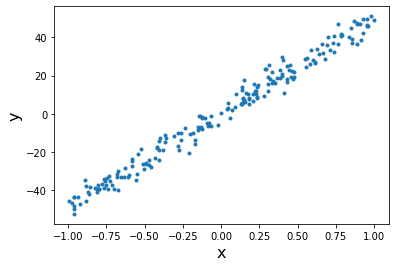
\includegraphics[width=.9\linewidth]{./figures/regression.png}
\end{figure}
\end{minipage}
\begin{minipage}{0.4\linewidth}
\begin{figure}
                        \centering
                        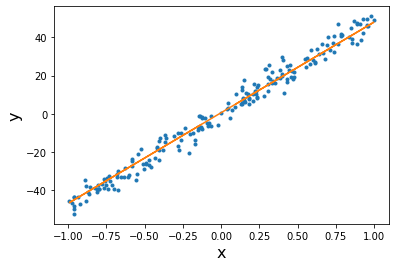
\includegraphics[width=.9\linewidth]{./figures/regression_example.png}
\end{figure}
\end{minipage}

\textbf{$D=1$ in all what follows}.
\end{frame}


\begin{frame}{Linear regression (with $D=1$)}
\vspace{-5mm}
\begin{itemize}
\item We have $N$ i.i.d. data points $\{(x_1, y_1), ..., (x_N, y_N)\}$ where $x_i\in \mathbb{R}$ $y_i\in \mathbb{R}$ for all $1 \leq i \leq N$.\\
\item Our linear model $f_{w, b}(x) = w * x + b$ has two parameters: $w \in \mathbb{R}$ and $b \in \mathbb{R}$.
\item We estimate these \emphbf{parameters} by minimizing \emphbf{mean squared error (MSE)} between model predictions and the actual data through \emphbf{gradient descent}.
\end{itemize}
\vsp
\pause
\textbf{Algorithm:}
\begin{itemize}
\item Randomly initialize the model parameters: $w_0 \in \mathbb{R}$ and $b_0 \in \mathbb{R}$.
\item Choose \emphbf{hyper-parameters}: learning rate $\alpha$ \& number of training steps $T$.
\item Repeat the following training steps $T$ times. At each step $t$ (from 0 to $T-1$):
\vspace{-3mm}
\begin{itemize}
\item Compute the MSE loss using the current value of $w_t$ and $b_t$: $\displaystyle \mathcal{L}(w_t, b_t) = \dfrac{1}{N} \sum_{i=1}^N \|f_{w_t, b_t}(x_i) - y_i  \|^2$
\item Compute the corresponding gradients: $\dfrac{\partial \mathcal{L}}{\partial w}(w_t, b_t)$ and $\dfrac{\partial \mathcal{L}}{\partial b}(w_t, b_t)$
\item Update parameters: $w_{t+1} = w_{t} - \alpha \dfrac{\partial \mathcal{L}}{\partial w}(w_t, b_t)$ and   $b_{t+1} = b_{t} - \alpha \dfrac{\partial \mathcal{L}}{\partial b}(w_t, b_t)$
\end{itemize}
\end{itemize}
Code? PyTorch?
\end{frame}


\begin{frame}[fragile]{Linear regression\\ How to generate data points?}

This is a ``toy task.'' We synthetically generate $N$ data points:
\begin{itemize}
\item For that, we start by setting the "true" $w^*$ and $b^*$ (that we choose).
\item We randomly sample $x_i$. Using that we compute $\hat{y}_i = w * x_i + b$.
\item Add a Gaussian noise: $y_i = \hat{y}_i + \epsilon_i$ with $\epsilon_i \sim \mathcal{N}(0, \sigma^2)$
where $\sigma$ is the standard deviation (that we choose).
\item We end up with noisy data points: $(x_i, y_i)$
\end{itemize}
\begin{python}
import numpy as np

def create_dataset(sample_size=10, sigma=0.1, w_star=1, b_star=1,
                   x_range=(-1, 1), seed=0):
    """Create data points for linear regression."""
    random_state = np.random.RandomState(seed)
    x_min, x_max = x_range
    x = random_state.uniform(x_min, x_max, (sample_size))
    y = x * w_star + b_star
    y += random_state.normal(0.0, sigma, (sample_size))

    return x, y

\end{python}
\end{frame}

\begin{frame}[fragile]{Linear regression (cont'd)\\ How to generate data points?}
% \vspace{-6mm}
\begin{itemize}
\item Generate the training data:
\end{itemize}
\begin{python}
num_samples = 200
sigma = 4
w_star = 50
X, y = create_dataset(
    sample_size=num_samples, sigma=sigma, w_star=w_star, seed=0)
\end{python}
\vsp
\begin{itemize}
\item From the same distribution, also sample the \emphbf{validation} data points using a different \emphbf{seed}:
\end{itemize}
\begin{python}
val_num_samples = 200
X_val, y_val = create_dataset(
    sample_size=num_samples, sigma=sigma, w_star=w_star, seed=42)
\end{python}
\end{frame}

\begin{frame}[fragile]{Linear regression (cont'd)\\ How to generate data points?}
% \vspace{-6mm}
\begin{itemize}
\item Visualize the data:
\end{itemize}
\begin{python}
import matplotlib.pyplot as plt

fig, ax = plt.subplots()
ax.set_xlabel("x", fontsize=16)
ax.set_ylabel("y", fontsize=16)

ax.plot(X, y, ".")
\end{python}
\begin{figure}
                        \centering
                        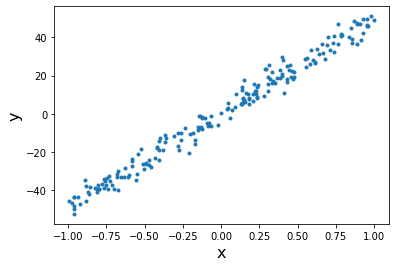
\includegraphics[width=.45\linewidth]{./figures/regression.png}
\end{figure}
\vspace{-5mm}
Check the documentation!
\end{frame}

\begin{frame}[fragile]{Linear regression, basic components}
\vspace{-6mm}
All necessary components are already implemented in PyTorch.
\begin{itemize}
\item We need a linear model $f$: $f_{\theta}(x) = w * x + b$\\
where $w \in \mathbb{R}$ and $b \in \mathbb{R}$ are the model parameters.
Build-in model in PyTorch is \codeb{torch.nn.Linear}.
\item We need the mean squared error:
\codeb{torch.nn.MSELoss}.
\item We update the model parameters using gradient descent.
The corresponding optimizer class is \codeb{torch.optim.SGD}
\end{itemize}
\begin{python}
import torch
import torch.nn as nn
import torch.optim as optim

DEVICE = torch.device("cuda:0" if torch.cuda.is_available()
                      else "cpu")

model = nn.Linear(1, 1)  # input dimension 1, and output dimension 1.
model = model.to(DEVICE)
loss_fn = nn.MSELoss()
learning_rate = 0.1
optimizer = optim.SGD(model.parameters(), lr=learning_rate)
\end{python}
\end{frame}

\begin{frame}[fragile]{Linear regression (cont'd)}
\vspace{-6mm}
Illustration of components (try on your own!):
\begin{itemize}
\item \codeb{torch.nn.Linear}.
\end{itemize}
\begin{python}
>>> import torch
>>> model = torch.nn.Linear(1, 1)
>>> model.weight
Parameter containing:
tensor([[-0.6464]], requires_grad=True)
>>> model.bias
Parameter containing:
tensor([-0.7324], requires_grad=True)
>>> x = torch.tensor([3.])
>>> model(x)
  # -0.6464 * 3. - 0.7324
tensor([-2.6717], grad_fn=<AddBackward0>)
\end{python}
\begin{itemize}
\item Recommendation: read documentation of \codeb{torch.nn.Linear}.
\item[-] e.g., how are the parameters initialized by default? 
\end{itemize}

\end{frame}

\begin{frame}[fragile]{Linear regression (cont'd)}
\vspace{-6mm}
\begin{itemize}
\item \codeb{torch.nn.MSELoss}.
\end{itemize}
\begin{python}
>>> import torch
>>> loss = torch.nn.MSELoss()
>>> a = torch.tensor([2.])
>>> b = torch.tensor([2.2])
>>> loss(a, b)
tensor(0.0400)
\end{python}
\begin{itemize}
\item \codeb{torch.optim.SGD}
\end{itemize}
\begin{python}
>>> import torch
>>> x = torch.tensor(2., requires_grad=True)
>>> z = x * x
>>> opt = torch.optim.SGD([x], lr=0.1)
>>> z.backward()
>>> opt.step()
>>> x
tensor(1.6000, requires_grad=True)
\end{python}
Again: \textbf{try on your own!} read documentation.
\end{frame}

\begin{frame}[fragile]{Linear regression (cont'd)}
\vspace{-6mm}
\begin{itemize}
\item Back to our regression problem.
\item The rest is to run the training loop.
\item But before that, data shape/dtype/device must be prepared as expected
by the function which will take them as input.
\end{itemize}

\begin{python}
X = X.reshape(num_samples, 1)  # shape expected by nn.Linear
X = torch.from_numpy(X)  # convert to torch.tensor
X = X.float()  # convert to float32 (from numpy double).
X = X.to(DEVICE)  # copy data to GPU.

# Same for other variables:
y = torch.from_numpy(y.reshape((num_samples, 1))).float().to(DEVICE)
X_val = torch.from_numpy(
  X_val.reshape((val_num_samples, 1))).float().to(DEVICE)
y_val = torch.from_numpy(
  y_val.reshape((val_num_samples, 1))).float().to(DEVICE)

\end{python}
\end{frame}

\begin{frame}[fragile]{Linear regression (cont'd)}
\vspace{-6mm}
Run the training loop.
\begin{python}
num_steps = 50  # We do 50 steps of gradient updates.

for step in range(num_steps):
    model.train()  # systematic: put model in 'training' mode.
    optimizer.zero_grad()  # systematic: start step w/ zero gradient.

    y_ = model(X)  # do prediction using the current model.
    loss = loss_fn(y_, y)  # compute error.
    print(f"Step {step}: train loss: {loss}")  # print train loss

    loss.backward()  # compute gradients.
    optimizer.step()  # update parameters

    # Eval on validation set
    model.eval()  # systematic: put model in 'eval' mode.
    # everything below does not contribute to gradient computation
    with torch.no_grad():
        y_ = model(X_val)
        val_loss = loss_fn(y_, y_val)
    print(f"Step {step}: val loss: {val_loss}") 

\end{python}
Or: \codeb{model.zero\_grad()} instead of \codeb{optimizer.zero\_grad()}.
\end{frame}

\begin{frame}[fragile]{Linear regression (cont'd)}
\vspace{-6mm}
Plot the resulting model:
\begin{python}
# Get the prediction from the final model.
model.eval()
with torch.no_grad():
    y_ = model(X)
fig, ax = plt.subplots()
ax.plot(X.cpu().numpy(), y.cpu().numpy(), ".")
ax.plot(X.cpu().numpy(), y_.cpu().numpy(), "-")

ax.set_xlabel("x", fontsize=16)
ax.set_ylabel("y", fontsize=16)
\end{python}
\begin{figure}
                        \centering
                        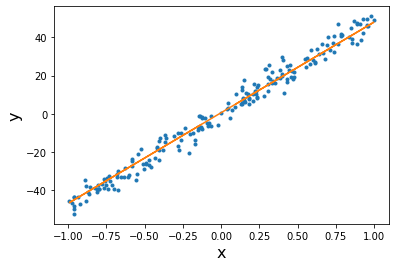
\includegraphics[width=.5\linewidth]{./figures/regression_example.png}
\end{figure}
\end{frame}


\begin{frame}[fragile]{Linear regression (cont'd)}
\vspace{-6mm}
We can also take a look at the final model parameters:
\begin{python}
>> model.weight
Parameter containing:
tensor([[47.3805]], device='cuda:0', requires_grad=True)
>> model.bias
Parameter containing:
tensor([0.5539], device='cuda:0', requires_grad=True)
\end{python}
\begin{itemize}
\item This was a simple example problem to illustrate some PyTorch functionalities.
\item A similar problem is to be solved in the \emphbf{Assignment 1}.
\item In the next lectures, we look into more details of components for building systems.
\end{itemize}
\end{frame}


\begin{frame}{A few words on \emphbf{Exercise 2 \& 3}}
\textbf{Now: Exercise 2}
\begin{itemize}
\item Objective: get familiar with PyTorch basics.
\end{itemize}
\vsp
\vsp
\emphbf{Next week: Assignment 1 (Exercise 3)}
\begin{itemize}
\item First assignment
\item Contributes to 15\% of the final grade.
\item Task: polynomial regression
\item You will be using many basic tools that you have learned:
\begin{itemize}
\item numpy random number generator
\item plot data points
\item ...
\end{itemize}
\end{itemize}
\end{frame}
% -----------------------------------------------------------------------
\subsection{Implementation of Systems}
\begin{frame}{Implementation of Systems}
\textbf{What do we need?} Reminder:
\vsp
\begin{itemize}
\item Dataset
\item Model
\item Loss
\item Optimizer
\item Multiple optimization steps (training loop).
\end{itemize}
\end{frame}

\begin{frame}[fragile]{Structure Preview: Sketch}
\vspace{-6mm}
\begin{python}
device = torch.device('cuda')  # 'cuda' for GPU.
dataset = MyDataset(...)
dataloader = DataLoader(dataset, ...) 

model = MyModel(...)
model = model.to(device)  # put the model params on device.
optimizer = torch.optim.SGD(model.parameters(), lr = 0.01)
loss_fn = Loss(...)

for i in range(10):  # Training loop for 10 epochs.
    for sample in dataloader:  # get batch.
        data = sample['data'].to(device)
        target = sample['target'].to(device)

        prediction = model(data)
        loss = loss_fn(prediction, target)

        optimizer.zero_grad() # reset the gradients
        loss.backward()
        optimizer.step()  # update params.
    # validation.
        # compute validation loss ...
        # save the intermediate model, ...
\end{python}
% training_loss += loss.item()
\end{frame}

\begin{frame}{Implementing datasets / dataloader}
For SGD, we need to generate data batches (i.e. randomly sampled training examples).\\
\vsp
\textbf{Two useful classes} in \code{torch.utils.data}
\begin{itemize}
\item \codeb{torch.utils.data.Dataset}: class for representing the dataset.
\item \codeb{torch.utils.data.Dataloader}: class for generating batches of data (does e.g. shuffling).
\end{itemize}
\vsp
Official tutorial: \link{https://pytorch.org/tutorials/beginner/data_loading_tutorial.html}
\end{frame}

\begin{frame}[fragile]{Dataset}
\vspace{-4mm}
\textbf{Three main methods:}
\begin{itemize}
\item \code{\_\_init\_\_(self)}
\item \code{\_\_getitem\_\_(self, index)}
\item \code{\_\_len\_\_(self)}
\end{itemize} 
\begin{python}
from torch.utils.data import Dataset, DataLoader

class RandomDataset(Dataset):

    def __init__(self, data_dim, num_data_points):
        self.len = num_data_points
        self.data = torch.randn(num_data_points, data_dim)

    def __getitem__(self, index):
        return self.data[index]

    def __len__(self):
        return self.len
\end{python}
\end{frame}

\begin{frame}[fragile]{Dataloader}
Generate batches.\\
Continue from the previous slides:
\begin{python}
input_dim = 10 
data_size = 1000
rand_dataset = RandomDataset(input_dim, data_size)

batch_size = 32
data_loader =
  DataLoader(dataset=rand_dataset,
             batch_size=batch_size, shuffle=True)

for i, data in enumerate(data_loader, 0):
    # each data contains 32 random samples of the data
    # data can then be to be fed to the model.
    ...
\end{python}
One can also specify a more specific way of sampling batches e.g. via \codeb{sampler} argument of \codeb{DataLoader}.
Alternatively: you could also implement your own data loader.
\end{frame}

\begin{frame}{Implementing models using PyTorch}
PyTorch \textbf{models} are regular Python class which inherits from \codeb{torch.nn.Module}\\
\vsp
\textbf{Two main methods}
\begin{itemize}
\item \codeb{\_\_init\_\_(self)}: define model components.
\item \codeb{forward(self, x)}: forward computation, given input $x$.
\end{itemize}
\end{frame}

\begin{frame}[fragile]{PyTorch Models, example}
\vspace{-8mm}
\begin{python}
import torch.nn as nn
import torch.nn.functional as F

class MyModel(nn.Module):

    def __init__(self, input_size, output_size):
        super(MyModel, self).__init__()
        self.fc = nn.Linear(input_size, output_size)

    def forward(self, input):
        output = self.fc(input)
        output = F.relu(output)
        return output
\end{python}
Note: model itself can contain \codeb{nn.Module} object, here \codeb{nn.Linear} a linear transformation layer.\\
These basic building blocks are already implemented; ready to be used.
\end{frame}

%\begin{frame}[fragile]{Put together, training example}
%\vspace{-8mm}
%\begin{python}
%import torch.nn as nn
%import torch.nn.functional as F
%
%class Net(nn.Module):
%    def __init__(self):
%        super(Net, self).__init__()
%        self.conv1 = nn.Conv2d(3, 6, 5)
%        self.pool = nn.MaxPool2d(2, 2)
%        self.conv2 = nn.Conv2d(6, 16, 5)
%        self.fc1 = nn.Linear(16 * 5 * 5, 120)
%        self.fc2 = nn.Linear(120, 84)
%        self.fc3 = nn.Linear(84, 10)
%\end{python}
%\end{frame}

\begin{frame}[fragile]{Checking model information}
\pause
\vspace{-6mm}
Continue from last slide.\\
\texttt{print} gives a decent overview:
% \begin{python}
%>>> model = MyModel(5, 2)
%>>> list(model.children())
%[Linear(in_features=5, out_features=2, bias=True)]
%\end{python}
\begin{python}
>>> model = MyModel(5, 2)
>>> print(model)
MyModel(
  (fc): Linear(in_features=2, out_features=5, bias=True)
)
\end{python}
\pause
Inspecting model parameters via \texttt{state\_dict()}:
\begin{python}
>>> for key, value in model.state_dict().items():
...    print(key)
...    print(value)
fc.weight
tensor([[ 0.1786,  0.4163, -0.0949,  0.0152,  0.4388],
        [-0.2598,  0.0871,  0.3840, -0.3750,  0.4289]])
fc.bias
tensor([0.0083, 0.1554])
\end{python}
%\pause
%\begin{python}
%>>> for module in model.named_modules():   # TODO check
%...   print(module)
%('', MyModel(
%  (fc): Linear(in_features=5, out_features=2, bias=True)
%))
%('fc', Linear(in_features=5, out_features=2, bias=True))
%\end{python}
\end{frame}

\begin{frame}[fragile]{Train vs. Evaluation Modes}
Some model components have different behaviors whether
it is in training or evaluation mode (e.g. dropout, batch normalization).
\pause
\vsp
\begin{itemize}
\item Run \codeb{model.train()} before training.
\item Run \codeb{model.eval()} before evaluation. 
\end{itemize}
\vsp
\pause
Also, to avoid modifying your model during evaluation,
you should everything under:
\begin{python}
with torch.no_grad():
    # evaluation
    ...
\end{python}
to prevent gradient computation (also saves memory).
\end{frame}

\begin{frame}[fragile]{Loss}
Different types of losses are available:
\begin{itemize}
\item \codeb{torch.nn.MSELoss}
\item \codeb{torch.nn.CrossEntropyLoss} (note: softmax is included in the loss computation)
\item etc...
\end{itemize}
\vsp
Illustration:
\begin{python}
>>> loss_fn = nn.MSELoss()
>>> predictions = torch.randn(3, 5, requires_grad=True)
>>> targets = torch.randn(3, 5)
>>> loss = loss_fn(predictions, targets)
>>> loss.backward()
\end{python}
\end{frame}

\begin{frame}[fragile]{Optimizer}
\vspace{-3mm}
Very much straightforward:
\begin{itemize}
\item Choose optimizer of your choice.\\
Most popular ones: \codeb{torch.optim.Adam} and \codeb{torch.optim.SGD}.
\item Do \codeb{optimizer.zero\_grad()} before backward computation.\\
Remember the gradients are accumulated.
\item Do \codeb{optimizer.step()}. It updates all params.
\end{itemize}
\begin{python}
optimizer = torch.optim.SGD(model.parameters(), lr = 0.01)

for sample in dataloader:
    data = sample['input'].to(device)
    target = sample['target'].to(device)
    prediction = model(data)
    loss = loss_fn(prediction, target)
    optimizer.zero_grad()  # reset gradients.
    loss.backward()
    optimizer.step()  # one step of update according to optimizer.
\end{python}
\end{frame}

\begin{frame}[fragile]{Saving \& Loading models}
\begin{itemize}
\item \codeb{torch.save}
\end{itemize}
\begin{python}
state = {'model_state' : model.state_dict(),
         'optimizer': optimizer.state_dict)}
torch.save(state, 'state.pt')
\end{python}
\vsp
\begin{itemize}
\item \codeb{torch.load}
\end{itemize}
\begin{python}
model = MyModel()
optimizer = optim.SGD(model_parameters(), lr=0.01)
checkpoint = torch.load('state.pt')
model.load_state_dict(checkpoint['model_state'])
optimizer.load_state_dict(checkpoint['optimizer_state'])
\end{python}
\vsp
Note: some optimizers also have some states which
must be stored, in order to resume training from
where it had been stopped. 
\end{frame}

\begin{frame}[fragile]{Monitoring training}
Finally, all pieces are essentially there!\\
\pause
\vsp
One last thing: \textbf{monitoring training process}.
\pause
\begin{itemize}
\item Training can take a long time. Depending on the task, it can take from a few days to a few months!\\ (fortunately not in our exercises.)
\pause
\item You would want to check the state of its progress by \textit{monitoring}
whether the training and validation losses are \textbf{going down}.
\pause
\item Also, you can detect very bad choices of (training) hyper-parameters, by checking the values of the training loss \textbf{just after a  few updates}!
\end{itemize}
$\rightarrow$ \emphbf{You will experience this in the exercises.}\\
\vsp
\vsp
\pause
Methods for monitoring:
\begin{itemize}
\item \textbf{Print the loss values} regularly, after each $n$ updates.
\item Use \textbf{visualization tools}: tensorboard, \textit{Weights \& Biases}, ...
\end{itemize}
\end{frame}

\begin{frame}[fragile]{Tensorboard}
\vspace{-5mm}
\begin{itemize}
\item Tool for visualizing and monitoring training.
\item Originally part of TensorFlow (Google).
\end{itemize}
\vsp
\pause
Basic idea:
\begin{itemize}
\item Add a few lines in your code to record the quantities of your interest in a log.
\item \texttt{tensorboard} provides visualization of the log (on a browser).
\end{itemize}
\pause
\begin{python}
from tensorboardX import SummaryWriter

writer = SummaryWriter(logdir='my-experiment/')

# ... inside the training loop ...
    # `train_steps` counts the training steps.
    # forward the model, compute loss etc
    writer.add_scalar('loss', loss, train_steps)
    # ...
    writer.add_scalar('train acc', train_acc, train_steps)
    # ... etc
\end{python}
(or \codeb{from torch.utils.tensorboard import SummaryWriter})
\end{frame}

\begin{frame}[fragile]{Tensorboard, illustration}
\begin{itemize}
\item You need to first install tensorboard: \codeb{pip install tensorboard}
\item Run \codeb{tensorboard --logdir my-experiment} on terminal.
\item This should give:\\ \texttt{TensorBoard 2.3.0 at http://localhost:6006/}
\item Paste it on your browser:
\end{itemize}
\begin{figure}
                        \centering
                        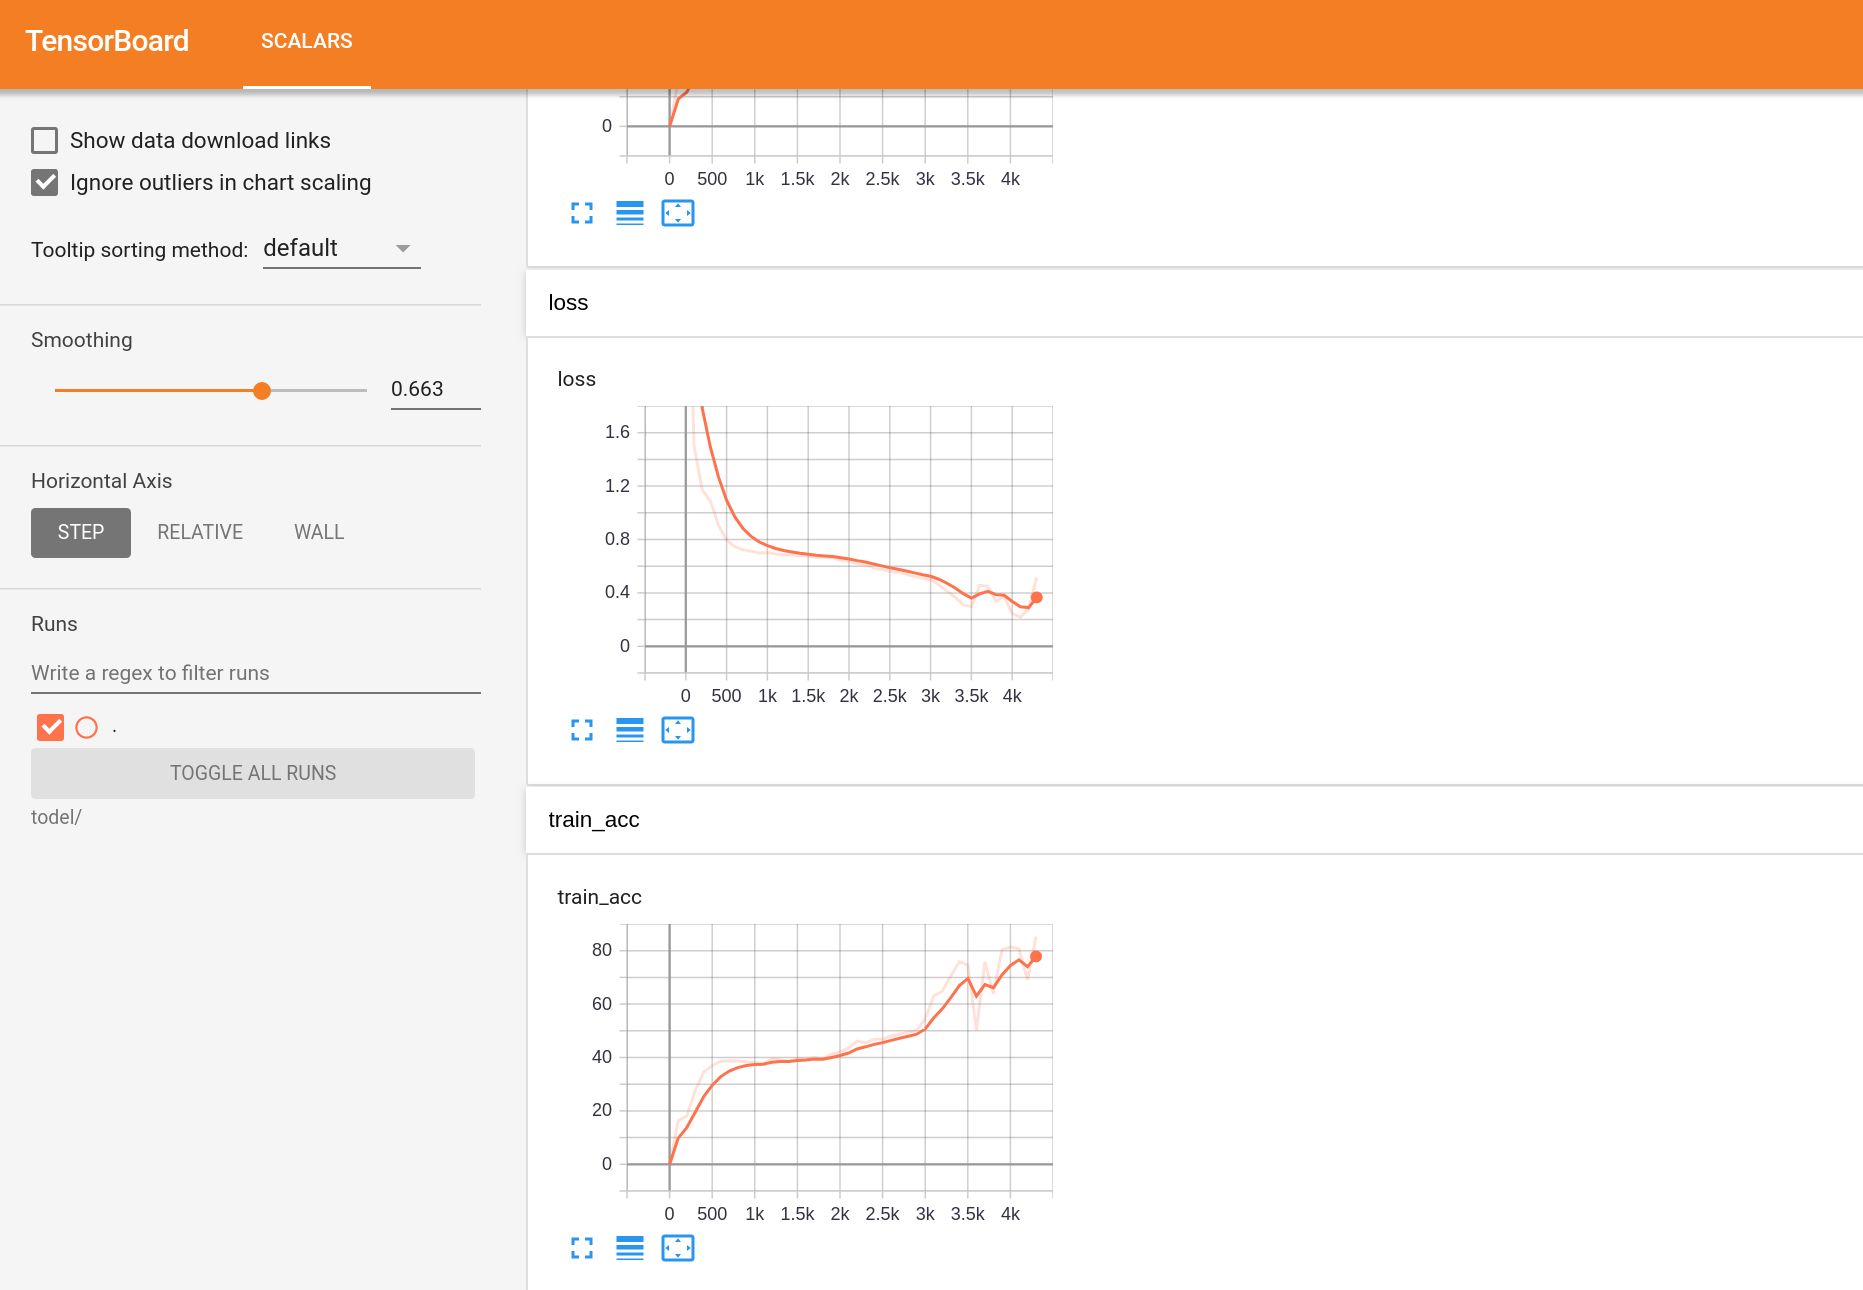
\includegraphics[width=.6\linewidth]{./figures/tensorboard.png}
% \vspace{-3mm}
\end{figure}
\end{frame}

%\begin{frame}{Put them all together!\\ example with linear regression}
%\TODO maybe directly MNIST with FF.
%\textbf{Regression task}:
%\begin{itemize}
%\item We have $N$ data points $\{(x_1, y_1), ..., (x_N, y_N)\}$ which are i.i.d.\\ $x_i\in \mathbb{R}^D$ $y_i\in \mathbb{R}$ for all $1 \leq i \leq N$.\\
%\item We want to find a function $f_{\theta}$ parametrized by $\theta$, which predicts well $y$ from $x$ for unseen $(x, y)$.
%\item Linear regression: use $f_{\theta}(x) = w . x + b$\\
%where $w \in \mathbb{R}^D$ and $b \in \mathbb{R}$ are model parameters. So $\theta = \{w, b\}$.
%\end{itemize}
%\end{frame}

\begin{frame}{Put them all together! Full example}
Let's consider \textbf{digit image classification} task using the MNIST dataset \citem{lecun1998mnist} and a two-layer \textbf{feed-forward neural network}:
\pause
\vsp
\begin{itemize}
\item Task: \textbf{classification} of images; each image is one handwritten digit (0 to 9).
\item[-] Input to the model: image.
\item[-] Output of the model: 10-dim vector, representing probability for each digit (10 classes).
\item[-] Can feed-forward models handle this problem? Yes.
\end{itemize}
\pause
\vsp
Basic statistics:
\begin{itemize}
\item 60\,K training images, 10\,K test images.
\item Dimension of each image: $\mathbb{R}^{28 \times 28}$, in black \& white (one channel),
\item[-] which can be reshaped to 784-dim vector, to input to the model.
\end{itemize}
\end{frame}

\begin{frame}[fragile]{Import packages... etc}
\vspace{-5mm}
\begin{python}
import torch
import torch.nn as nn
import torchvision
import torchvision.transforms as transforms
\end{python}

\begin{python}
device = torch.device(
    "cuda:0" if torch.cuda.is_available() else "cpu")
\end{python}

\begin{python}
# Hyper-parameters
# to specify model:
input_size = 784
hidden_size = 512
num_classes = 10

# for training:
num_epochs = 5
batch_size = 128
learning_rate = 0.001
momentum = 0.9
\end{python}
\end{frame}

\begin{frame}[fragile]{Create datasets/dataloader}
MNIST is standard dataset: you can directly get it from \code{torchvision}.
\begin{python}
# Datasets
train_set = torchvision.datasets.MNIST(
    root='./data', train=True, transform=transforms.ToTensor(), 
    download=True)

test_set = torchvision.datasets.MNIST(
    root='./data', train=False, transform=transforms.ToTensor())

# Dataloaders
train_loader = torch.utils.data.DataLoader(
    dataset=train_set, batch_size=batch_size, shuffle=True)

test_loader = torch.utils.data.DataLoader(
    dataset=test_set, batch_size=batch_size, shuffle=False)

\end{python}
\end{frame}

\begin{frame}[fragile]{Define model}
\begin{itemize}
\item We use a basic \textbf{feed-forward} neural network with 2 layers (one hidden vector) with the ReLU activation function.
\item[-] The dimension $d$ of the hidden vector is the \textbf{model hyper-parameter}.
\item[-] The input and output dimensions are specified by the problem.
\vsp
\pause
\item Input image $x \in \mathbb{R}^{784}$ (reshaped 28x28 image).
\item The first layer transforms $x \in \mathbb{R}^{784}$ to a hidden vector $h \in \mathbb{R}^{d}$:
\[
h = \ReLU(W_1x + b_1) = \max(W_1x + b_1, 0)
\]
$W_1 \in \mathbb{R}^{d \times 784}$ and $b_1 \in \mathbb{R}^{d}$ are \textbf{trainable/model parameters}.
\pause
\item The output layer transforms $h \in \mathbb{R}^{d}$ to a vector $y \in \mathbb{R}^{10}$
(size = number of classes = 10 digit):
\[
y = W_2h + b_2
\]
$W_2 \in \mathbb{R}^{10 \times d}$ and $b_2 \in \mathbb{R}^{10}$ are \textbf{trainable/model parameters}.
%\item $W_1 \in \mathbb{R}^{d \times 784}$, $W_2 \in \mathbb{R}^{10 \times d}$, $b_1 \in \mathbb{R}^{d}$, and $b_2 \in \mathbb{R}^{10}$
%are the trainable parameters of the model.
\pause
\item[-] Softmax function transforms the logit $y$ to a probability distribution: for $i \in \{0,..., 9\}$
\[
p(i|x) = \softmax(y)_i
\]
\end{itemize}
\end{frame}

\begin{frame}[fragile]{Define model, implementation}
\begin{python}
class FFModel(nn.Module):

    def __init__(self, input_size, hidden_size, num_classes):
        super(FFModel, self).__init__()
        self.fc1 = nn.Linear(input_size, hidden_size) 
        self.fc2 = nn.Linear(hidden_size, num_classes)  
    
    def forward(self, x):
        # Assume linealized input: here `images.view(-1, 28*28)`.
        out = self.fc1(x)
        out = F.relu(out)
        out = self.fc2(out)
        # second layer does not need activation function;
        # softmax is computed by cross entropy loss.
        return out
\end{python}
\end{frame}

\begin{frame}[fragile]{Create model, loss, optimizer}
\begin{python}
# Create model
model = FFModel(input_size, hidden_size, num_classes)
model = model.to(device)  # put all model params on GPU.

# Create loss and optimizer
loss_fn = nn.CrossEntropyLoss()

optimizer = optim.SGD(
    model.parameters(), lr=learning_rate, momentum=momentum)
\end{python}
\end{frame}

\begin{frame}[fragile]{Training}
\vspace{-5mm}
\begin{python}
# Training
for epoch in range(num_epochs):
    model.train()  # Set model in train mode.
    for i, (images, labels) in enumerate(train_loader):
        # shape of images is (B, 1, 28, 28).
        images = images.view(-1, 28*28)  # reshape to (B, 784).
        images = images.to(device)  # copy data to GPU.
        labels = labels.to(device)  # shape (B).

        outputs = model(images)  # shape (B, 10).
        loss = loss_fn(outputs, labels)

        optimizer.zero_grad()  # reset gradients.
        loss.backward()  # compute gradients.
        optimizer.step()  # update parameters.
        
        # here, print the current value of loss...
        # saving model checkpoint... to be done in Exercise!
\end{python}
\end{frame}

\begin{frame}[fragile]{Evaluation}
\vspace{-5mm}
\begin{python}
# Evaluation
with torch.no_grad():
    correct = 0
    total = 0
    model.eval()  # Set model in eval mode. Don't forget!
    for images, labels in test_loader:
        images = images.view(-1, 28*28)
        images = images.to(device)
        labels = labels.to(device)  # shape (B)
        outputs = model(images)  # shape (B, num_classes)
        # 'outputs' are logits (unnormalized log prob).
        # Model prediction is the class which has the highest
        # probability according to the model,
        # i.e. the class which has the highest logit value:
        _, predicted = outputs.max(dim=1)
        # predicted.shape: (B)
        total += labels.size(0)
        correct += (predicted == labels).sum().item()
    test_acc = 100 * correct / total

print(f'Test accuracy is: {test_acc} %')
\end{python}

%\begin{python}
%# Evaluation
%with torch.no_grad():
%    correct = 0
%    total = 0
%    model.eval()  # Set model in eval mode. Don't forget!
%    for images, labels in test_loader:
%        images = images.view(-1, 28*28)
%        images = images.to(device)
%        labels = labels.to(device)  # shape (B)
%        outputs = model(images)  # shape (B, num_classes)
%        # 'outputs' are logits (unnormalized log prob).
%        # Model prediction is the class which has the highest
%        # probability according to the model,
%        # i.e. the class which has the highest logit value:
%        _, predicted = torch.max(outputs.data, 1)
%        # predicted.shape: (B)
%        total += labels.size(0)
%        correct += (predicted == labels).sum().item()
%    test_acc = 100 * correct / total
%
%print(f'Test accuracy is: {test_acc} %')
%\end{python}
\end{frame}


\begin{frame}{Not covered in this example}
\begin{itemize}
\item Preparation of \emphbf{validation} dataset!\\ Crucial for tuning \emphbf{hyper-parameter}.
\item Hyper-parameter tuning.
\item Monitoring of intermediate model performance during training \& saving model parameters.
\item ... we will see more refinements to in the chapter after next one!
\end{itemize}
\vsp
You will do these in \emphbf{Exercise 4}!
\end{frame}

%\begin{frame}{Alternative frameworks}
%Libraries:
%TensorFlow, JAX, MXNet,
%High-level frameworks:
%keras,
%Even higher...
%fairseq etc...
%Why PyTorch?
%recent Popularity, simplicity, mention OpenAI.
%\end{frame}

%\begin{frame}{Deep Learning libraries}
%Libraries:
%TensorFlow, JAX, MXNet,
%High-level frameworks:
%keras,
%Even higher...
%fairseq etc...
%\end{frame}

\begin{frame}{Excursions: C++ API}
\textbf{Beyond the scope of this lab.} \\
\vsp
When it is needed to go beyond Python?
\vsp
\begin{itemize}
\item To write custom operations in C++ to optimize some
special operations/models in terms of speed or memory consumption.\\
Official example: \textit{long long-term memory}
\link{https://pytorch.org/tutorials/advanced/cpp_extension.html}
\item To deploy models in C++/production code: you trained your model using code in Python but want to use the trained model in other code written in C++. Example Tesla?
\link{https://pytorch.org/tutorials/advanced/cpp_export.html}
\end{itemize}
\end{frame}

\begin{frame}{Summary}
\textbf{What have we learned?}
\begin{itemize}
\item Basics of Python+PyTorch.
\item Basic implementation of main components of deep learning workflow using PyTorch.
\item Many examples.
\end{itemize}
\vsp
\textbf{Coming up next...}
\begin{itemize}
\item What kind of neural networks should we consider for different problems?
\item How are they implemented in PyTorch?
\item ...
\end{itemize}
\end{frame}
